\section{Direct Dimensionality Reduction} 

  Dimensionality reduction is used for many purposes, such as preprocessing data, visualizing it, or encoding it in a sparser, more efficient way. 

  \subsection{Principal Component Analysis} 
    
    PCA finds low dimensional approximations to the data by projecting the data onto linear subspaces. 

    \begin{definition}[Principal Component Analysis]
      Let $X \in \mathbb{R}^d$ and $\mathcal{L}_k$ denote all $k$-dimensional linear subspaces. The $k$th principal subspace is 
      \begin{equation}
        \ell_k = \argmin_{\ell \in \mathcal{L}_k} \mathbb{E} \big( \min_{y \in \ell} ||\Tilde{X} - y||^2 \big)
      \end{equation}
      where $\Tilde{X} = X - \mu$ and $\mu = \mathbb{E}[X]$. To parse this, let's fix a subspace $\ell$. Then, the normalized data $\Tilde{X}$ is a random vector and the minimum distance of $\Tilde{X}$ onto the subspace $\ell$ is the inner min term. Taking the expectation of that gives us the expected distance of the data onto the subspace. The principal subspace is the subspace that minimizes this expected distance. The dimension reduced version of $X$ is then $T_k (X) = \mu + \mathrm{proj}_{\ell_k} X$. 
    \end{definition}

    Note that this is in fact different from linear regression as it minimizes the expected \textit{orthogonal distance} to the subspace, rather than the residual distance to the subspace as in linear regression. 

    \begin{figure}[H]
      \centering
      \begin{subfigure}[b]{0.3\textwidth}
      \centering
        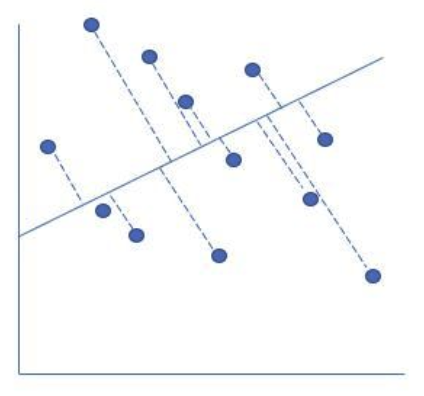
\includegraphics[width=\textwidth]{img/pca_ortho.png}
        \caption{PCA minimizes the orthogonal distance to the subspace. }
      \end{subfigure}
      \begin{subfigure}[b]{0.3\textwidth}
      \centering
        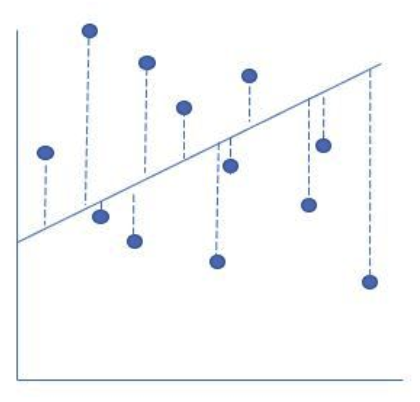
\includegraphics[width=\textwidth]{img/lin_reg_vert.png}
        \caption{Linear regression minimizes the residual distance to the subspace.} 
      \end{subfigure}
      \caption{PCA vs Linear Regression}
      \label{fig:pca_lin_reg}
    \end{figure}

    There is a very nice way to calculate this principal subspace. 

    \begin{theorem}[Calculating the Principal Subspace] 
      Given our data matrix $X \in \mathbb{R}^{n \times d}$, we take the SVD of it. 
      \begin{equation}
        X = U \Sigma V^T
      \end{equation}
      where $\Sigma$ contains the singular values of $X$ in decreasing order. Then $\ell_k$ is the subspace spanned by the columns $v_1, v_2, \ldots, v_k$ of $V$. Furthermore, 
      \begin{equation}
        T_k (X) = \mu + \sum_{j=1}^k \beta_j v_j , \text{ where } \beta_j = \langle X - \mu, v_j \rangle
      \end{equation}
      Note that this is really just equivalent to calculating the eigendecomposition of $\hat{\Sigma} = X^T X$. 
    \end{theorem}

    Now a question arises: how do we know that this sample decomposition is a good approximation to the true decomposition? It comes from the fact that the sample covariance $\hat{\Sigma}$ is a good approximation of the true covariance $\Sigma$, which we will later prove using concentration of measure. 

    \begin{theorem}[Risk]
      The risk satisfies 
      \begin{equation}
        R(k) = \mathbb{E}[|| X - T_k (X) ||^2 ] = \sum_{j=k+1}^d \lambda_j 
      \end{equation}
    \end{theorem}

    It is essential that you plot the spectrum in decreasing order. This allows you to analze how well PCA is working. People often use the ``elbow'' technique to determine where to choose $K$, and we value 
    \begin{equation}
      \frac{\sum_{j=1}^k \lambda_j}{\sum_{j=1}^d \lambda_j} 
    \end{equation}
    accounts for the \textbf{variance explained}, which should be high with $K$ low. If you have to go out to dimension $K=50$ to explain $90\%$ of the variance, then PCA is not working. It may not work because of many reasons, such as there being nonlinear structure within the data. 

    It turns out that the elements of $\hat{\Sigma}$ are close entry-wise to those of $\Sigma$. But if this is true, then does it mean that the eigenvalues of the sample covariance matrix are close to the true eigenvalues of the covariance matrix? It turns out that the answer is no, and we need a proper metric to satisfy this assumption. The metric, as we can guess from linear algebra, is the operator norm, and we will show some results from matrix perturbation theory. 

    \begin{definition}[Operator Norm]
      The \textbf{operator norm} of a matrix $A$ is defined as 
      \begin{equation}
        ||A|| = \sup_{x \neq 0} \frac{||Ax||}{||x||} 
      \end{equation}
    \end{definition}

    \begin{lemma}[]
      It turns out that 
      \begin{equation}
        ||\hat{\Sigma} - \Sigma|| = O_p \bigg( \frac{1}{\sqrt{n}} \bigg)
      \end{equation}
    \end{lemma}

    \begin{theorem}[Weyl's Theorem]
      If $\hat{\Sigma}$ and $\Sigma$ are close in the operator norm, then their eigenvalues are close. 
      \begin{equation}
        ||\hat{\Sigma} - \Sigma|| = O_p \bigg( \frac{1}{\sqrt{n}} \bigg) \implies |\hat{\lambda}_j - \lambda_j| = O_p \bigg( \frac{1}{\sqrt{n}} \bigg) 
      \end{equation}
    \end{theorem}

    This only talks about their eigenvalues, but this does not necessarily imply that the eigenvalues are close. We need an extra condition. 

    \begin{theorem}[David-Kahan Theorem]
      If $\hat{\Sigma}$ and $\Sigma$ are close in the operator norm, and if the eigenvectors of $\Sigma$ are well-conditioned, then the eigenvectors of $\hat{\Sigma}$ are close to the eigenvectors of $\Sigma$. More specifically, 
      \begin{equation}
        ||\hat{v}_j - v_j|| \leq \frac{2^{3/2} ||\hat{\Sigma} - \Sigma||}{\lambda_j - \lambda_{j+1}}
      \end{equation}
    \end{theorem}

    \subsubsection{Kernel PCA}

      \begin{definition}[Kernel PCA]
        Let $N_i$ be the neighborhood around $X_i$. Then, we want to find a mapping $W: \mathbb{R}^n \rightarrow \mathbb{R}^k$ that minimizes 
        \begin{equation}
          \min_{W} \sum_{i=1}^n \bigg| \bigg| X_i - \sum_{j \in N_i} W_{ij} X_j \bigg| \bigg|^2 \text{ where } \sum_{j} W_{ij} = 1
        \end{equation}
        We can constrain the weights in $W$ so that anything that is not in the neighborhoods are $0$. 
      \end{definition}

  \subsection{Multi-Dimensional Scaling}

    Again, we want to reduce our dimension, but the goal is slightly different from PCA. 

    \begin{definition}[Multi-Dimensional Scaling]
      Given our data $X \in \mathbb{R}^d$, we want to construct a linear map $T: \mathbb{R}^d \rightarrow \mathbb{R}^k$ such that it preserves the pairwise differences between the data points. That is, we want to minimize the following loss function 
      \begin{equation}
        \min_{T} \sum_{i \neq j} \big( d_{\mathbb{R}^k}(T(x_i), T(x_j)) - d_{\mathbb{R}^d}(x_i, x_j) \big)
      \end{equation}
      where $d_{V}$ is a distance metric in the space $V$. 
    \end{definition}

    Note that we can easily modify this formulation to preserve other structures, such as dot products, weights between distances, or different types of metrics in each space. It turns out that when the distance metric is the Euclidean L2 distance, then the solution to this linear map turns out to be PCA. This may be a more intuitive way to think about PCA, since we're trying to preserve the pairwise distances between the data points. 

    \begin{theorem}[Equivalence of Classical MDS and PCA]
      If the distance metric is the Euclidean L2 distance, then the solution to the MDS problem is equivalent to PCA. That is, 
      \begin{equation}
        T_k = \argmin_{T} \sum_{i \neq j} \big( ||T(x_i) - T(x_j)||^2 - ||x_i - x_j||^2 \big)
      \end{equation}
    \end{theorem}

    Generally, if you don't use classical MDS, then you will get a different answer than PCA and there doesn't exist a closed form solution, so you'll have to minimize this numerically. 

    \begin{example}[Non Classical MDS]
      The loss 
      \begin{equation}
        \sum_{i \neq j}  \big( ||T(x_i) - T(x_j)|| - ||x_i - x_j|| \big)^2 
      \end{equation}
      does not give the same solution as PCA. 
    \end{example}

  \subsection{Isomap} 

    Isomap is a bit different in the way that it tries to capture more of the global structure of the data, which brings advantages and disadvantages. It is simply a modification of MDS but with geodesic distances. 

    \begin{definition}[Isomap]
      You start off with the point cloud, but with every point, $X_i$, you find the local neighborhood $N_i$ and you make a weighted graph over the whole dataset in the high dimensional space. Then, the distance between any two arbitrary points is the weighted sum of the path between them, calculated by Dijkstra's algorithm. Intuitively, this is an approximation of the geodesic distance between these two points on a manifold. Call this distance $d_G$. Then, we simply do MDS by minimizing 
      \begin{equation}
        \min_{T} \sum_{i \neq j} \big( d_{\mathbb{R}^k}(T(x_i), T(x_j)) - d_G(x_i, x_j) \big)
      \end{equation}

      \begin{figure}[H]
        \centering 
        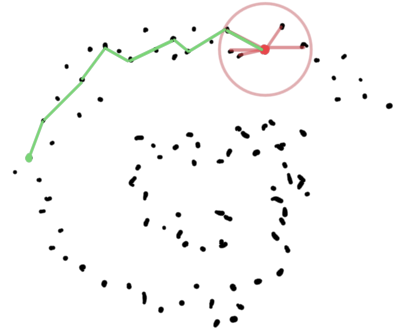
\includegraphics[scale=0.4]{img/isomap.png}
        \caption{The classical example is the spiral manifold. The data lies in this manifold, and the geodesic distance helps us gain an accurate distance metric within this data. } 
        \label{fig:isomap}
      \end{figure}
    \end{definition}

    The problem with this is that it is very sensitive to noise. For example, if we had a few points lying between the spirals, then the geodesic distance between the two spirals would be very small, and so the MDS would try to bring them closer together.  

    \begin{figure}[H]
      \centering 
      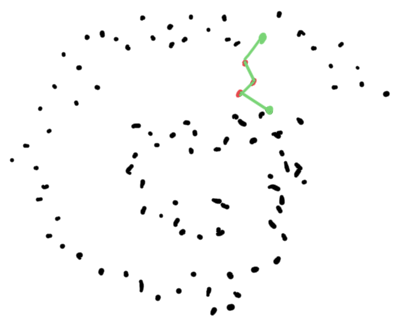
\includegraphics[scale=0.4]{img/isomap_problem.png}
      \caption{With extra noisy points (red), the geodesic distance can get corrupted.} 
      \label{fig:isomap_problem}
    \end{figure}

    To fix this, we use \textit{diffusion maps}, which looks at all possible paths between two points and looks at some average of them, which increases robustness. 

  \subsection{Local Linear Embedding} 

    PCA and MDS are linear embedding methods. Let's move onto nonlinear ones. The first nonlinear models that we work with again use the idea of locality (remember kernel regression). You have data that is globally nonlinear, but if you look at a point and its local neighborhood around it, then it is approximately linear since we assume that it lives in some smooth manifold. 

    \begin{figure}[H]
      \centering 
      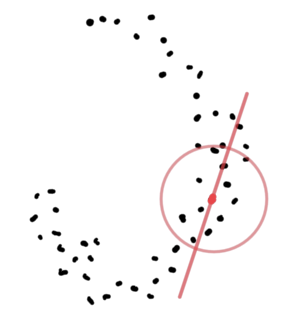
\includegraphics[scale=0.4]{img/local_linear_embedding.png}
      \caption{Local linear embedding assumes that the data is locally linear. } 
      \label{fig:local_linear_embedding}
    \end{figure}

    The concept of neighborhood can be defined in two ways. You can either just fix an $\epsilon$ and take the $\epsilon$-ball around each point $x_i$. Or you can fix a $k$ and take the $k$ nearest neighbors of each point. The general idea of using kernel PCA is to take a local neighborhood of the data and construct some linear approximation of it. 

  \subsection{UMAP}

  \subsection{t-SNE}

